\capitulo{3}{Conceptos teóricos}

Se sintetizarán a continuación algunos de los conceptos teóricos más relevantes para la correcta comprensión del documento.

\section{Apendizaje automático}

Se denomina aprendizaje automático a aquella rama de la inteligencia artificial cuyo objetivo es desarrollar métodos que permitan que un algoritmo mejore su rendimiento mediante la experiencia y procesado de datos. Consecuentemente, los modelos entrenados realizarán predicciones cada vez más precisas como resultado del algoritmo implementado.

Dentro del aprendizaje automático se diferencian tres grandes grupos en función del tipo de entrada que sea consumida: el aprendizaje supervisado (datos etiquetados), el no supervisado (datos no etiquetados) y el semisupervisado (datos etiquetados y no etiquetados), siendo esta última categoría objeto de estudio en este proyecto de investigación. 

\subsection{Aprendizaje semisupervisado}

Como se ha mencionado anteriormente, se denomina aprendizaje semisupervisado a aquel conjunto de algoritmos que utiliza datos etiquetados y no etiquetados para realizar tareas de aprendizaje. Inicialmente, se pueden diferenciar dos categorías\cite{engelen2020surveyOnSemiSupervised}: los métodos inductivos, cuyo objetivo principal es construir un clasificador que genere predicciones para cualquier entrada y los métodos transductivos, cuyo poder de predicción está limitado a los objetos utilizados en la fase de entrenamiento.


\begin{figure}[h]
\caption{Clasificación sugerida por \cite{engelen2020surveyOnSemiSupervised}}
\centering
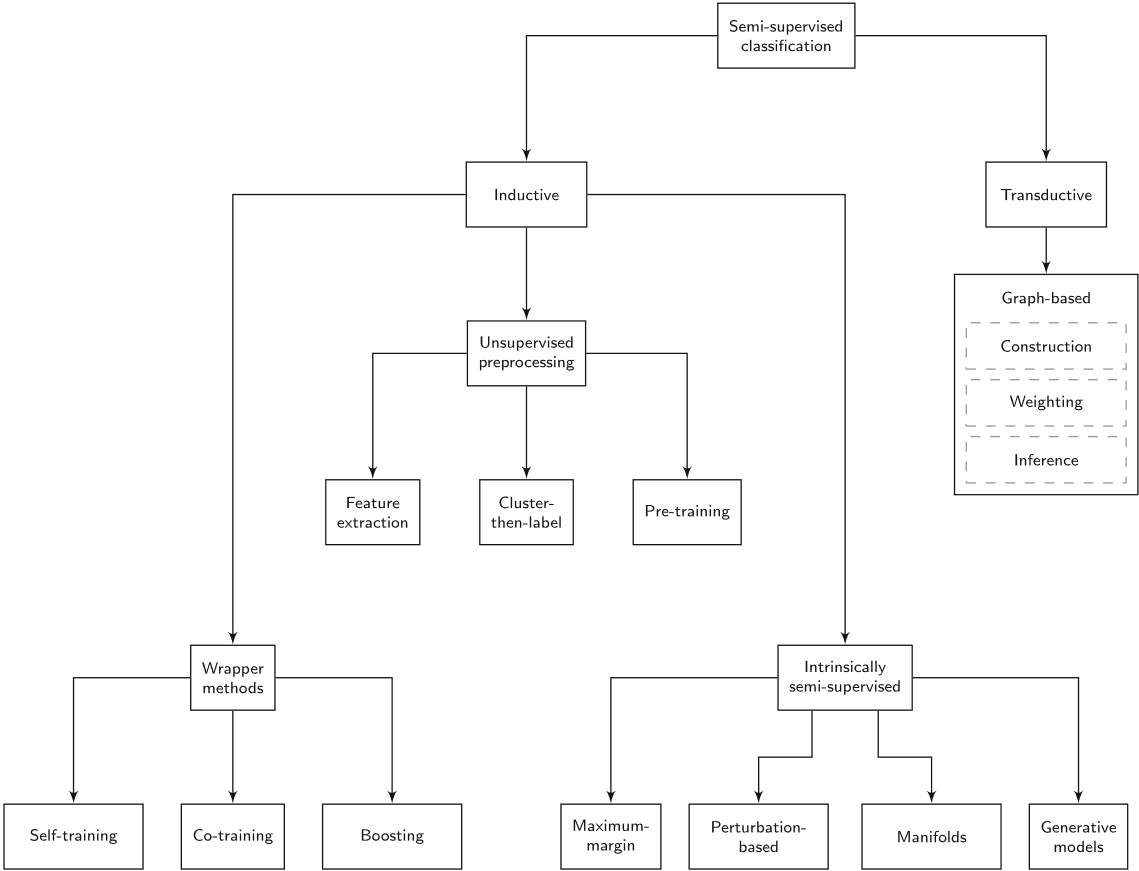
\includegraphics[width=\textwidth]{esquemaHoos}
\end{figure}

Prescindiendo de los métodos transductivos por ser menos versátiles y útiles en nuestro propósito, los métodos inductivos se subdividen en tres grupos \cite{engelen2020surveyOnSemiSupervised}: \textit{wrapper methods} (o métodos de envoltura), \textit{unsupervised preprocessing} y \textit{intrinsically semi-supervised}, siendo materia de estudio los métodos de envoltura. 


\subsubsection{Métodos de envoltura}

Estos modelos utilizan uno o más clasificadores que son entrenados iterativamente con los datos etiquetados de entrada, además de con datos pseudoetiquetados. Se denomina pseudoetiquetado a aquellos datos que inicialmente no estaban etiquetados, pero acabaron estándolo por iteraciones previas de los clasificadores.

Consecuentemente, el procedimiento consta de dos fases que se repiten en cada iteración: el entrenamiento y el pseudoetiquetado. Durante el entrenamiento, los clasificadores se alimentan de datos etiquetados (o pseudoetiquetados). En la fase de pseudoetiquetado, se utilizan datos no etiquetados para que sean procesados por los clasificadores previamente entrenados. 

Dentro de esta categoría, se pueden diferenciar tres grandes grupos: \textit{self-training}, que utilizan únicamente un clasificador, \textit{co-training}, que utilizan más de uno y los \textit{pseudo-labelled boosting methods}, que construyen clasificadores individuales que se alimentan de las predicciones más fiables. Se estudiará más en profundidad los métodos \textit{co-training}.

\subsubsection{Co-training y Co-forest}

En estos algoritmos, varios clasificadores son entrenados iterativamente utilizando datos etiquetados y añadiendo las predicciones (resultados) más certeras al conjunto para ser utilizadas en las siguientes iteraciones. Para que los clasificadores sean capaces de generar información distinta, generalmente se divide el conjunto de entrada según alguna característica (no siendo estrictamente necesario).

El llamado \textit{co-forest}, es un modelo dentro del \textit{co-training}. En su desarrollo, se utilizan árboles de decisión (a mayor número mejor resultado), que son entrenados utilizando los datos etiquetados. En cada iteración, además, se añade al conjunto de datos nuevos elementos pseudoetiquetados. Estos elementos son el resultado de los elementos comunes (nuevas etiquetas) del resto de árboles en la fase anterior, y se usan durante una fase de entrenamiento. Sin embargo, se eliminan una vez se ha completado (la siguiente iteración se realiza inicialmente sólo con los datos etiquetados, etc.), consiguiendo así resultados certeros.









